\documentclass[11pt]{report}

%-------------------------------------------------------------------------------------------------%

% PAQUETES

\usepackage[a4paper, right = 0.8in, left = 0.8in, top = 0.8in, bottom = 0.8in]{geometry}
\usepackage[utf8]{inputenc}
\usepackage[spanish]{babel}
\usepackage{amsmath,amsfonts,amssymb,amsthm}
\usepackage{multicol}
\usepackage{fouriernc}
\usepackage{enumitem}
\usepackage{mathtools} % Solo uso \underbracket
\usepackage{cellspace, tabularx, booktabs} % Líneas del título
\usepackage{parskip}
\usepackage{pdfpages}
\usepackage{cancel}

%-------------------------------------------------------------------------------------------------%

% AJUSTES GENERALES

\setlist[enumerate]{label={\textit{\alph*})}}

\makeatletter % Para quitar el espacio adicional que el paquete parskip añade al principio y al final de una demostración
\renewenvironment{proof}[1][\proofname]{\par
  \pushQED{\qed}%
  \normalfont \topsep\z@skip % <---- changed here
  \trivlist
  \item[\hskip\labelsep
        \itshape
    #1\@addpunct{.}]\ignorespaces
}{%
  \popQED\endtrivlist\@endpefalse
}
\makeatother

%-------------------------------------------------------------------------------------------------%

% COMANDOS PERSONALIZADOS

\newcommand{\N}{\mathbb N}
\newcommand{\Z}{\mathbb Z}
\newcommand{\Q}{\mathbb Q}
\newcommand{\R}{\mathbb R}
\newcommand{\C}{\mathbb C}

\newcommand{\pars}[1]{\left( #1 \right)} % Paréntesis de tamaño automático
\newcommand{\comment}[1]{}

%-------------------------------------------------------------------------------------------------%

% EJERCICIOS Y SOLUCIONES

\newtheorem{ejercicio}{Ejercicio}
\addto\captionsspanish{\renewcommand*{\proofname}{Solución}}

%-------------------------------------------------------------------------------------------------%

\begin{document}

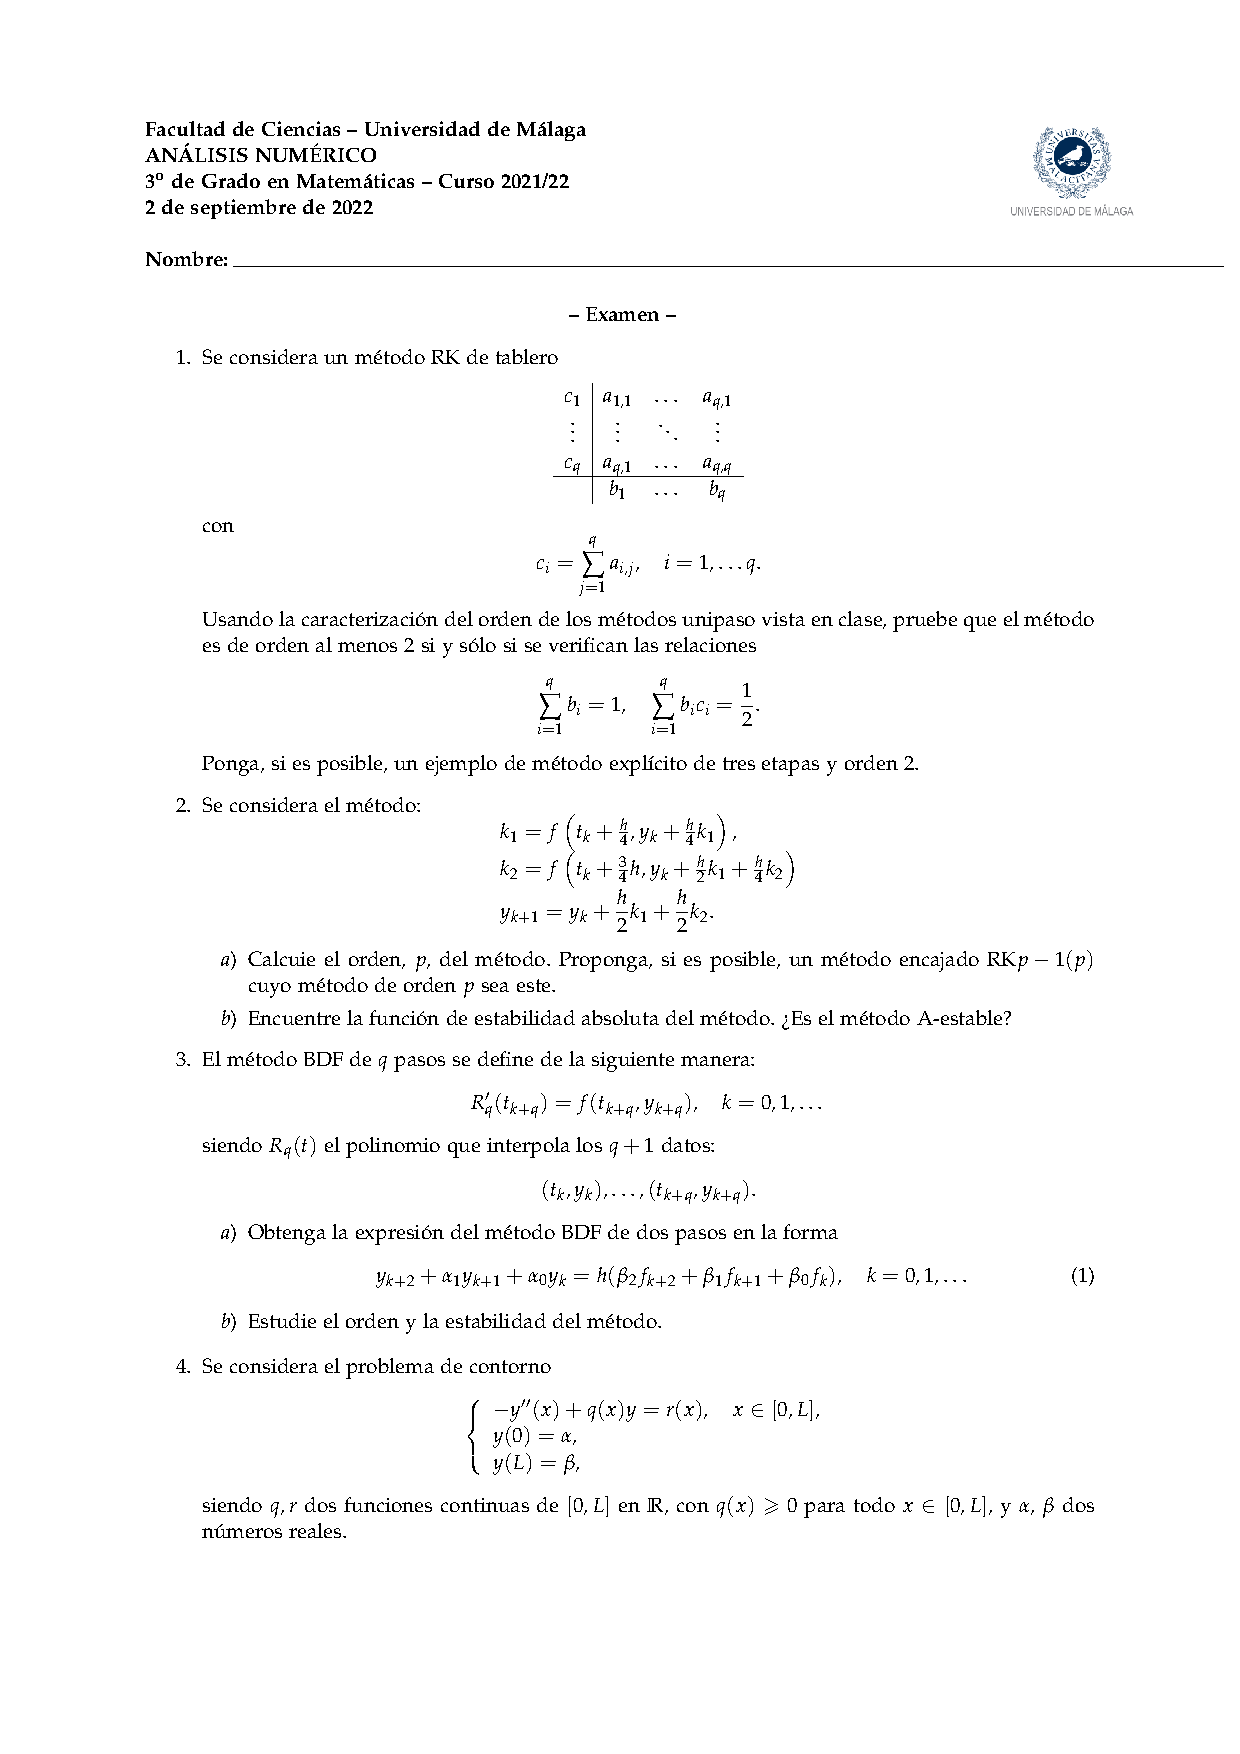
\includepdf[pages=-]{an_examen_2022-09.pdf}

%-------------------------------------------------------------------------------------------------%

% TÍTULO

\begin{center}

	\textbf{$-$ Resolución $-$}

\end{center}

%-------------------------------------------------------------------------------------------------%

\textbf{1.} La función incremento del método RK con el tablero del enunciado es 
\[\Phi(t,y,h) = \sum_{i=1}^q b_if(t^{(i)}, y^{(i)}),\]
donde, para cada $i \in \{1,2,\mathellipsis,q\}$,
\[t^{(i)} = t + c_ih, \qquad \qquad y^{(i)} = y+h\sum_{j=1}^q a_{i,j}f(t^{(j)},y^{(j)})\]
son funciones de $(t,y,h)$. Por tanto,
\[\Phi(t,y,0) = \sum_{i=1}^qb_if(t,y) = f(t,y)\sum_{i=1}^q b_i\]
Además,
\[
    \frac{\partial \Phi}{\partial h}(t,y,h) = \sum_{i=1}^qb_i \frac{d}{dh}f(t^{(i)},y^{(i)}) = \sum_{i=1}^qb_i \left(\frac{\partial f}{\partial t}(t,y,h)\frac{\partial t^{(i)}}{\partial h}(t,y,h)+\frac{\partial f}{\partial y}(t,y,h)\frac{\partial y^{(i)}}{\partial h}(t,y,h)\right) \tag{$\ast$}
\]
Por un lado,
\[\frac{\partial t^{(i)}}{\partial h}(t,y,h) = c_i\]
Por otro lado,
\[\frac{\partial y^{(i)}}{\partial h}(t,y,h) = \sum_{j=1}^qa_{i,j}f(t^{(j)},y^{(j)}) + h \frac{d}{dh}\sum_{j=1}^q a_{i,j}f(t^{(j)},y^{(j)})\]
En consecuencia,
\[\frac{\partial t^{(i)}}{\partial h}(t,y,0) = c_i, \qquad \qquad \frac{\partial y^{(i)}}{\partial h}(t,y,0) =\sum_{j=1}^qa_{i,j}f(t,y) = c_if(t,y),\]
donde se ha usado que en $h=0$ es $f(t^{(j)},y^{(j)}) = f(t,y)$ y que
\[c_i = \sum_{j=1}^q a_{i,j}\]
Volviendo a $(\ast)$,
\[\begin{aligned}[t]\frac{\partial \Phi}{\partial h}(t,y,0) &= \sum_{i=1}^qb_i \left(\frac{\partial f}{\partial t}(t,y,0)\frac{\partial t^{(i)}}{\partial h}(t,y,0)+\frac{\partial f}{\partial y}(t,y,0)\frac{\partial y^{(i)}}{\partial h}(t,y,0)\right) \\
    &=  \sum_{i=1}^qb_i \left(\frac{\partial f}{\partial t}(t,y,0)c_i+\frac{\partial f}{\partial y}(t,y,0)c_if(t,y)\right) \\
    &= \sum_{i=1}^q b_ic_i \left(\frac{\partial f}{\partial t}(t,y,0)+f(t,y)\frac{\partial f}{\partial y}(t,y,0)\right) \\
    &=\sum_{i=1}^q b_ic_i f^{(1)}(t,y)
\end{aligned}\]
Ahora bien, se sabe que el método es de orden al menos $2$ si y solo si
\[\Phi(t,y,0) = f(t,y), \qquad \qquad \frac{\partial \Phi}{\partial h}(t,y,0) = \frac{1}{2}f^{(1)}(t,y)\]
Pero hemos probado que
\[\Phi(t,y,0) = f(t,y) \sum_{i=1}^q b_i, \qquad \qquad \frac{\partial \Phi}{\partial h}(t,y,0) = \sum_{i=1}^q b_ic_i f^{(1)}(t,y),\]
concluyéndose que el método es de orden al menos $2$ si y solo si 
\[\sum_{i=1}^qb_i = 1, \qquad \qquad \sum_{i=1}^q b_ic_i = \frac{1}{2}\]
En consecuencia, un método RK explícito de tres etapas y orden $2$ debe ser de la forma

\begin{center}
    \setlength\extrarowheight{2.5pt}
    \begin{tabular}{c|ccc}
        0 & 0 & 0 & 0 \\
        1 & 1 & 0 & 0 \\
        1 & 1/2  & 1/2  & 0 \\ \hline
        & 1/2 & 1/4 & 1/4
    \end{tabular}
    \end{center}

En efecto, este método verifica
\[c_i = \sum_{j=1}^3a_{i,j}, \ i \in \{1,2,3\}, \qquad \qquad \sum_{i=1}^3 b_i = 1, \qquad \qquad \sum_{i=1}^3b_ic_i = \frac{1}{2}\]

\textbf{2.} Nótese que
\[\textstyle k_1 = f\left(t_k+\frac{h}{4},y_k+\frac{h}{4}k_1\right) \iff y_k+\frac{h}{4}k_1 = y_k+\frac{h}{4}f\left(t_k+\frac{h}{4},y_k+\frac{h}{4}k_1\right)\]
Llamando $y_k^{(1)} = y_k+\frac{h}{4}k_1$, se tiene
\[\textstyle y_k^{(1)} = y_k+\frac{h}{4}f(t_k+\frac{h}{4},y_k^{(1)})\]
Por otra parte,
\[\textstyle k_2 = f\left(t_k+\frac{3}{4}h, y_k+\frac{h}{2}k_1+\frac{h}{4}k_2\right) \iff y_k+\frac{h}{2}k_1+\frac{h}{4}k_2 = y_k+\frac{h}{2}k_1+\frac{h}{4}f\left(t_k+\frac{3}{4}h, y_k+\frac{h}{2}k_1+\frac{h}{4}k_2\right)
\]
Llamando $y_k^{(2)} = y_k+\frac{h}{2}k_1+\frac{h}{4}k_2$, se tiene
\[\textstyle
    y_k^{(2)} =  y_k+\frac{h}{2}k_1+\frac{h}{4}f\left(t_k+\frac{3}{4}h, y_k+\frac{h}{2}k_1+\frac{h}{4}k_2\right) =  y_k+\frac{h}{2}f\left(t_k+\frac{h}{4},y_k^{(1)}\right)+\frac{h}{4}f\left(t_k+\frac{3}{4}h, y_k^{(2)}\right)
\]
Por último,
\[\textstyle y_{k+1}=y_k+\frac{h}{2}k_1+\frac{h}{2}k_2 = y_k+\frac{h}{2}f\left(t_k+\frac{h}{4},y_k^{(1)}\right)+\frac{h}{2}f\left(t_k+\frac{3}{4}h,y_k^{(2)}\right)\]
En consecuencia, las tres ecuaciones del método se pueden escribir como 
\[ \textstyle \begin{cases}
     y_k^{(1)}  &\hspace{-3mm}= y_k+\frac{h}{4}f(t_k+\frac{h}{4},y_k^{(1)}) \\[5pt]
     y_k^{(2)} &\hspace{-3mm}= y_k+h\bigl(\frac{1}{2}f(t_k+\frac{h}{4},y_k^{(1)})+\frac{1}{4}f(t_k+\frac{3}{4}h,y_k^{(2)})\bigr) \\[5pt]
     y_{k+1} &\hspace{-3mm}= y_k+h\bigl(\frac{1}{2}f(t_k+\frac{h}{4},y_k^{(1)})+\frac{1}{2}f(t_k+\frac{3}{4}h,y_k^{(2)})\bigr) \\
\end{cases} \]
Se trata de un método RK con tablero de Butcher

\begin{center}
    \setlength\extrarowheight{2.5pt}
    \begin{tabular}{c|cc}
        1/4 & 1/4 & 0 \\
        3/4 & 1/2  & 1/4 \\ \hline
        & 1/2 & 1/2
    \end{tabular}
    \end{center}

\begin{enumerate}
    \item Estudiemos el orden del método. Sean
    \[B = \left(\begin{array}{c}
        1/2 \\
        1/2
    \end{array}\right) \qquad \qquad E= \left(\begin{array}{c}
        1 \\
        1
    \end{array}\right) \qquad \qquad C = \left(\begin{array}{cc}
        1/4 & 0 \\
        0 & 3/4
    \end{array}\right) \qquad \qquad A=\left(\begin{array}{cc}
        1/4 & 0 \\
        1/2 & 1/4
    \end{array}\right)\]
    Se tiene que
    \[B^tE = \left(\begin{array}{cc}
        1/2 & 1/2
    \end{array}\right)\left(\begin{array}{c}
        1 \\
        1
    \end{array}\right) =1,\]
    luego el método es de orden $1$. Además,
    \[B^tAE = \left(\begin{array}{cc}
        1/2 & 1/2
    \end{array}\right)\left(\begin{array}{cc}
        1/4 & 0 \\
        1/2 & 1/4
    \end{array}\right)\left(\begin{array}{c}
        1 \\
        1
    \end{array}\right) = \left(\begin{array}{cc}
        3/8 & 1/8
    \end{array}\right)\left(\begin{array}{c}
        1 \\
        1
    \end{array}\right) = \frac{1}{2},\]
    así que el método es de orden $2$. Seguimos:
    \[B^tC^2E = \left(\begin{array}{cc}
        1/2 & 1/2
    \end{array}\right)\left(\begin{array}{cc}
        1/4 & 0 \\
        0 & 3/4
    \end{array}\right)\left(\begin{array}{cc}
        1/4 & 0 \\
        0 & 3/4
    \end{array}\right)\left(\begin{array}{c}
        1 \\
        1
    \end{array}\right) = \left(\begin{array}{cc}
        1/8 & 3/8
    \end{array}\right)\left(\begin{array}{c}
        1/4 \\
        3/4
    \end{array}\right) = \frac{5}{16} \neq \frac{1}{3} \]
    Esto indica que el método no es de orden $3$, así que es de orden exactamente $2$.
    \item La función de estabilidad absoluta viene dada por 
    \[\begin{aligned}[t] R(\hat{h}) &= \frac{|I-\hat{h}A+\hat{h}EB^t|}{|I-\hat{h}A|} = \left|\begin{array}{cc}
    1-\hat{h}/4 & 0 \\
    -\hat{h}/2 & 1-\hat{h}/4
    \end{array}\right|^{-1}\left|\begin{array}{cc}
        1-\hat{h}/4+\hat{h}/2 & \hat{h}/2 \\
        -\hat{h}/2+\hat{h}/2 & 1-\hat{h}/4+\hat{h}/2
    \end{array}\right| \\
    &=\left|\begin{array}{cc}
        1-\hat{h}/4 & 0 \\
        -\hat{h}/2 & 1-\hat{h}/4
        \end{array}\right|^{-1}\left|\begin{array}{cc}
            1+\hat{h}/4 & \hat{h}/2 \\
           0 & 1+\hat{h}/4
        \end{array}\right| = \frac{(1+\hat{h}/4)^2}{(1-\hat{h}/4)^2} = \frac{(4+\hat{h})^2}{(4-\hat{h})^2}
    \end{aligned}\]
    Sea $\hat{h}=x+iy \in \C^-$. Entonces
    \[\begin{aligned}[t]
        |R(\hat{h})| < 1 \iff |4+\hat{h}|^2 < |4-\hat{h}|^2 \iff (4+x)^2+y^2 < (4-x)^2+y^2 \iff 16+x^2+8x < 16+x^2-8x
    \end{aligned}\]
    Esto último es siempre cierto por ser $x<0$, así que $\C^- \subset D_A$ y por tanto el método es $A$-estable.
\end{enumerate}

\textbf{3. }

\begin{enumerate}
    \item El polinomio que interpola los datos
    \[(t_k,y_k),(t_{k+1},y_{k+1}),(t_{k+2},y_{k+2})\]
    es
    \[R(t)=\widetilde{R}\left(\frac{t-t_{k+2}}{h}\right),\]
    donde
    \[\begin{aligned}[t]
        \widetilde{R}(s)&=\sum_{j=0}^2 \nabla^jy_{k+2}\binom{s+j-1}{j} = y_{k+2}\binom{s-1}{0} +(y_{k+2}-y_{k+1})\binom{s}{1}+(y_{k+2}-2y_{k+1}+y_k)\binom{s+1}{2} \\
        &= y_{k+2}+(y_{k+2}-y_{k+1})s+\frac{1}{2}(y_{k+2}-2y_{k+1}+y_k)s(s+1) \\ &= y_{k+2}+(y_{k+2}-y_{k+1})s+\frac{1}{2}(y_{k+2}-2y_{k+1}+y_k)s^2+\frac{1}{2}(y_{k+2}-2y_{k+1}+y_k)s \\
        &= y_{k+2}+\left(\frac{3}{2}y_{k+2}-2y_{k+1}+\frac{1}{2}y_k\right)s+\frac{1}{2}\left(y_{k+2}-2y_{k+1}+y_k\right)s^2
    \end{aligned}
    \]
    Por la regla de la cadena,
    \[R'(t) = \frac{1}{h}\widetilde{R}'\left(\frac{t-t_{k+2}}{h}\right)\]
    En particular,
    \[R'(t_{k+2}) = \frac{1}{h}\widetilde{R}'(0) = \frac{1}{h}\left(\frac{3}{2}y_{k+2}-2y_{k+1}+\frac{1}{2}y_k\right)\]
    Por tanto, la expresión del método BDF de dos pasos es
    \[\frac{3}{2}y_{k+2}-2y_{k+1}+\frac{1}{2}y_k = hf_{k+2}, \qquad k = 0,1,\mathellipsis\]
    Equivalentemente,
    \[y_{k+2}-\frac{4}{3}y_{k+1}+\frac{1}{3}y_k = \frac{2h}{3}f_{k+2}, \qquad k = 0,1,\mathellipsis\]
    \item El primer polinomio característico del método es
    \[\rho(z)=z^2-\frac{4}{3}z+\frac{1}{3},\]
    cuyas raíces son $1$ y $\frac{1}{3}$. Las raíces de $\rho$ son de módulo menor que $1$ y las que son de módulo $1$ son simples, así que el método es estable. Estudiemos el orden. En primer lugar,
    \[\sum_{j=0}^2 \alpha_j = 1-\frac{4}{3}+\frac{1}{3} = 0\]
    Además,
    \[\sum_{j=0}^2\alpha_j j = -\frac{4}{3}+2 = \frac{2}{3}, \qquad \qquad \sum_{j=0}^2 \beta_j =\frac{2}{3},\]
    luego el método es de orden $1$. Y como
    \[\sum_{j=0}^2 \alpha_jj^2 = -\frac{4}{3}+4 = \frac{8}{3}, \qquad \qquad 2\sum_{j=0}^q \beta_jj = 2 \cdot \frac{2}{3} \cdot 2 = \frac{8}{3},\]
    entonces el método es de orden $2$. Sin embargo,
    \[\sum_{j=0}^2 \alpha_jj^3 = -\frac{4}{3}+8 = \frac{20}{3}, \qquad \qquad 3 \sum_{j=0}^2\beta_jj^2= 3 \cdot \frac{2}{3} \cdot 2^2 = 8 \neq \frac{20}{3},\]
    así que el método es de orden exactamente 2.
\end{enumerate}

\textbf{4. }

\begin{enumerate}
    \item Consideremos la fórmula de derivación numérica
    \[y''(\bar{x}) \approx D_3^2(y) = \frac{y(\bar{x}+h)-2y(\bar{x})+y(\bar{x}-h)}{h^2}\]
    En particular, para $i = 1,2,\mathellipsis,N$,
    \[y''(x_i) \approx D_3^2(y) = \frac{y(x_{i+1})-2y(x_i)+y(x_{i-1})}{h^2}\]
    Llamemos $u_i$ a la aproximación de $y(x_i)$ para cada $i = 1,2,\mathellipsis,N$, mientras que $u_0 = \alpha$, $u_{N+1} = \beta$. Entonces
    \[y''(x_i) \approx \frac{u_{i+1}-2u_i+u_{i-1}}{h^2}\]
    Sustituyendo estas aproximaciones en el problema se obtiene un método adecuado para aproximar la solución de dicho problema:
    \[\left\{ \begin{alignedat}{1}
        u_0 &= \alpha, \\
        \frac{u_{i+1}-2u_i+u_{i-1}}{h^2} &= q(x_i)u_i- r(x_i), \qquad i = 1,2,\mathellipsis,N, \\
        u_{N+1} &= \beta
    \end{alignedat} \right.\]
    \item Se va a tratar de transformar este método en un sistema de $N$ ecuaciones con $N$ incógnitas. La ecuación del sistema para $i = 1$ es, usando que $u_0 = \alpha$,
    \[\frac{u_2-2u_1+\alpha}{h^2} = q(x_1)u_1-r(x_1),\]
    o, equivalentemente, 
    \[\left(-2-h^2q(x_1)\right)u_1+u_2 = -h^2r(x_1)-\alpha\]
    Y para $i = N$, usando que $u_{N+1}=\beta$,
    \[\frac{\beta-2u_N+u_{N-1}}{h^2} = q(x_N)u_N-r(x_N),\]
    es decir,
    \[u_{N-1}+\left(-2-h^2q(x_N)\right)u_N = -h^2r(x_N)-\beta\]
    Por tanto, el método se escribe de forma equivalente como
    \[\left\{ \begin{alignedat}{1}
        \left(-2-h^2q(x_1)\right)u_1+u_2 &= -h^2r(x_1)-\alpha, \\
        \frac{u_{i+1}-2u_i+u_{i-1}}{h^2} &= q(x_i)u_i- r(x_i), \qquad i = 2,3,\mathellipsis,N-1, \\
        u_{N-1}+\left(-2-h^2q(x_N)\right)u_N &= -h^2r(x_N)-\beta,
    \end{alignedat} \right.\]
    o lo que es lo mismo,
    \[\left\{ \begin{alignedat}{1}
    \left(-2-h^2q(x_1)\right)u_1+u_2 &= -h^2r(x_1)-\alpha, \\
    u_{i-1}+\left(-2-h^2q(x_i)\right)u_i+u_{i+1} &= -h^2r(x_i), \qquad i = 2,3,\mathellipsis,N-1, \\
    u_{N-1}+\left(-2-h^2q(x_N)\right)u_N &= -h^2r(x_N)-\beta,
    \end{alignedat} \right.\]
    En forma matricial,
    \[AU=F,\]
    donde la matriz de coeficientes es
    \[A =\left(\begin{array}{cccccc}
        -2-h^2q(x_1) & 1 & 0 & \mathellipsis & 0 & 0 \\
        1 & -2-h^2q(x_2) & 1 & \mathellipsis & 0 & 0 \\
        \vdots & \vdots & \vdots & \ddots & \vdots & \vdots \\
        0 & 0 & 0 & \mathellipsis & -2-h^2q(x_{N-1}) & 1 \\
        0 & 0 & 0 & \mathellipsis & 1 & -2-h^2q(x_N)
    \end{array}\right)\]
    Esta matriz es simétrica, y como es tridiagonal con elementos diagonales negativos, entonces es definida negativa.
\end{enumerate}

\end{document}